\section{Introduction}
Data processing is an important step of many scientific studies. Type and size of data as well as the type of processing can determine the processing method. In seismological studies, we mostly deal with numerical data with different customized processing. In many cases, users write a function in a programming language (e.g. MATLAB\textsuperscript{\textregistered}, Python, C, Fortran) and process the data. Depending on the type of data and processing, we may need several steps of processing data in a project. Also we may have to change a parameter and repeat the processing several times.  Writing down the processing steps is a good practice to avoid confusion, keep track of the processing, and be able to return back and look for the probable bugs in case of wrong results. However, since it is not automated, you may unintentionally skip one step of processing or forget to properly document it. Even with complete documentation, in the case of finding the problem in processing steps, you need to repeat the whole process and go through all the steps. \\
Developing a data analysis package could be an excellent alternative to applying customized processing functions on massive data sets. In this short note, I present how to develop a data processing package. This note is not about the methods of data processing, or getting and cleaning data, or even programming. It presents how to use shell script to make your process faster, more accurate, and trackable. If you have  scripts in a different programming language and you are using those scripts repeatedly to process data, you may find this document helpful. The idea of having a data processing package is not novel. People mostly define such a structure in their projects. The goal of this note is to make this process easy to understand.\\
 Shell scripts (e.g. Unix shell) are robust computer program for handling files and folders. In this short note, I explain how to use shell scripts to mange the input and output files, and report any problem during the processing if necessary. The core function could be written in any programming language. Extra steps are required to use MATLAB in unix, so the following example show how to do this. However, the method is applicable to other programming languages with lower complexity. In summary, shell script prepares  data with a required format and name at the right time and right place to the core function and receive the results at the right time and right place to pass to other program or archive it.\\
Having a basic knowledge of programming in MATLAB and shell is necessary to understand this note. In the next two sections we will discuss the basic commands of shell and MATLAB. 

\begin{figure} [ht]
\centering
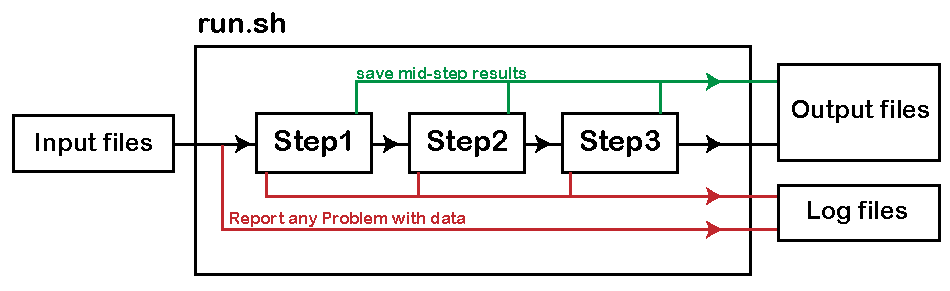
\includegraphics[scale=0.8]{figures/pdf/Figure01.pdf} 
\caption{Schematic of a data processing package.}
\label{fig:structure}
\end{figure}



